\documentclass{beamer}

\mode<presentation> {
%\usetheme{AnnArbor}
%\usetheme{Antibes}
%\usetheme{Bergen}
%\usetheme{Berkeley}
%\usetheme{Berlin}
%\usetheme{Boadilla}
%\usetheme{CambridgeUS}
%\usetheme{Copenhagen}
%\usetheme{Darmstadt}
%\usetheme{Dresden}
%\usetheme{Frankfurt}
%\usetheme{Goettingen}
%\usetheme{Hannover}
%\usetheme{Ilmenau}
%\usetheme{JuanLesPins}
%\usetheme{Luebeck}
\usetheme{Madrid}
%\usetheme{Malmoe}
%\usetheme{Marburg}
%\usetheme{Montpellier}
%\usetheme{PaloAlto}
%\usetheme{Pittsburgh}
%\usetheme{Rochester}
%\usetheme{Singapore}
%\usetheme{Szeged}
%\usetheme{Warsaw}

%\usecolortheme{albatross}
\usecolortheme{beaver}
%\usecolortheme{beetle}
%\usecolortheme{crane}
%\usecolortheme{dolphin}
%\usecolortheme{dove}
%\usecolortheme{fly}
%\usecolortheme{lily}
%\usecolortheme{orchid}
%\usecolortheme{rose}
%\usecolortheme{seagull}
%\usecolortheme{seahorse}
%\usecolortheme{whale}
%\usecolortheme{wolverine}
%\setbeamertemplate{footline}
%{
%	\leavevmode%
%	\hbox{%
%		\begin{beamercolorbox}[wd=.333333\paperwidth,ht=2.25ex,dp=1ex,center]{author in head/foot}%
%			\usebeamerfont{author in head/foot}\insertshortauthor
%		\end{beamercolorbox}%
%		\begin{beamercolorbox}[wd=.46\paperwidth,ht=2.25ex,dp=1ex,center]{title in head/foot}%
%			\usebeamerfont{title in head/foot}\insertshorttitle
%		\end{beamercolorbox}%
%		\begin{beamercolorbox}[wd=.2\paperwidth,ht=2.25ex,dp=1ex,right]{date in head/foot}%
%			\usebeamerfont{date in head/foot}
%			\insertframenumber{}% / \inserttotalframenumber
%			\hspace*{2ex} 
%	\end{beamercolorbox}}%
%	\vskip0pt%
%}
}

\usepackage{graphicx} % Allows including images
\usepackage{booktabs} % Allows the use of \toprule, \midrule and \bottomrule in tables
\usepackage{amsmath}
\usepackage{amsfonts}
\usepackage{ifthen}
\usepackage{amssymb}
\usepackage{amsbsy}
\usepackage{bm}
\usepackage{ulem}
\usepackage{float}
\usepackage{latexsym}
\usepackage{comment}
\usepackage{graphicx}
\usepackage{amstext}
\usepackage{latexsym}
\usepackage{arydshln}
\usepackage{longtable}
\usepackage{enumerate}
\usepackage{multirow}
\usepackage{cases}
\usepackage{geometry}
\usepackage{mathtools}
\usepackage{subeqnarray}
\usepackage{textcomp}
\usepackage{hyperref}
%\usepackage{subfigure}
\usepackage{url}
\usepackage{threeparttable}
\usepackage{xr}
\usepackage{multirow}
\usepackage{wrapfig}
\usepackage{lscape}
\usepackage{rotating}
\usepackage{subcaption}
\usepackage{epstopdf}
\usepackage{verbatim}
\usepackage{xcolor}
\usepackage[sort&compress]{natbib}
\usepackage{bm}


\newcommand{\bA}{\mathbf{A}}
\newcommand{\bB}{\mathbf{B}}
\newcommand{\bD}{\mathbf{D}}
\newcommand{\bF}{\mathbf{F}}
\newcommand{\bI}{\mathbf{I}}
\newcommand{\bLambda}{{\bm\Lambda}}
\newcommand{\bOmega}{{\bm\Omega}}
\newcommand{\bM}{\mathbf{M}}
\newcommand{\bN}{\mathbf{N}}
\newcommand{\bphi}{{\bm\phi}}
\newcommand{\bpsi}{{\bm\psi}}
\newcommand{\brho}{{\bm\rho}}
\newcommand{\bvarphi}{{\bm\varphi}}
\newcommand{\bW}{\mathbf{W}}
\newcommand{\sT}{\mathrm{T}}
\newcommand{\bZ}{\mathbf{Z}}
\newcommand{\shalf}{\mbox{{\footnotesize$\frac{1}{2}$}}}



\setbeamertemplate{theorems}[numbered]
\newtheorem{prop}{Proposition}
\let\oldframe\frame
\renewcommand{\frame}{%
\oldframe
\let\olditemize\itemize
\renewcommand\itemize{\olditemize\addtolength{\itemsep}{10pt}}%
}



%----------------------------------------------------------------------------------------
%	TITLE PAGE
%----------------------------------------------------------------------------------------


\title[Hierarchical Spatial FW Model for MET]{A Hierarchical Spatial Finlay-Wilkinson Model for Analysis of Multi-Environment Field Trials}

\author[Guo, X., Dutta, S., Nettleton, D.]{Xingche Guo, Somak Dutta, Dan Nettleton}
\institute[ISU]{Dept. of Statistics, Iowa State University}
\date[JSM, 2019]{Joint Statistical Meetings, 2019}

\AtBeginSection[]{
	\begin{frame}
		\vfill
		\centering
		\begin{beamercolorbox}[sep=8pt,center,shadow=true,rounded=true]{title}
			\usebeamerfont{title}\insertsectionhead\par%
		\end{beamercolorbox}
		\vfill
	\end{frame}
}





\begin{document}
\renewcommand{\inserttotalframenumber}{18}
\begin{frame}
\titlepage
\end{frame}

%\begin{frame}
%	\frametitle{Overview}
%	\tableofcontents
%\end{frame}



\begin{frame}
	\frametitle{The Genomes to Fields (G2F) Initiative}
	\begin{figure}[H]
		\centering
		
\includegraphics[width = 0.65\textwidth]{g2f_demo.png}
	\end{figure}	
	copyright:	\url{https://www.genomes2fields.org}
\end{frame}


\begin{frame}
	\frametitle{Multi-Environment Field Trial Analysis for G2F Data}
	\begin{itemize}
	\item Initially, we focus on a subset of 24 \textbf{environments}.
	\item We have \textbf{yield recorded for 10,971 field plots} with known \textbf{spatial locations}.
	\item A total of \textbf{1,105 hybrids} are planted in approximately 10 plots on average.
	\item Hybrid \textbf{genotypes at $\sim$1M genomic locations} are available.
	\item To characterize environments, weather stations provide \textbf{time-indexed measurements for 10 weather variables}, and several \textbf{soil variables} are available.
	\end{itemize}	
\end{frame}




\begin{frame}
	\frametitle{Finlay-Wilkinson (FW) Model}
	\begin{itemize}
	\item Finlay-Wilkinson (FW) model \citep{finlay1963analysis}: 
	$$y_{ijk} = \mu + g_i + h_j + b_i h_j + e_{ijk},$$
 \item For genotype $i$, FW model becomes a \textbf{linear model} with intercept $\mu + g_i$ and slope $b_i + 1 $.
	\end{itemize}		
	\pause
		\begin{figure}[H]
		\centering
		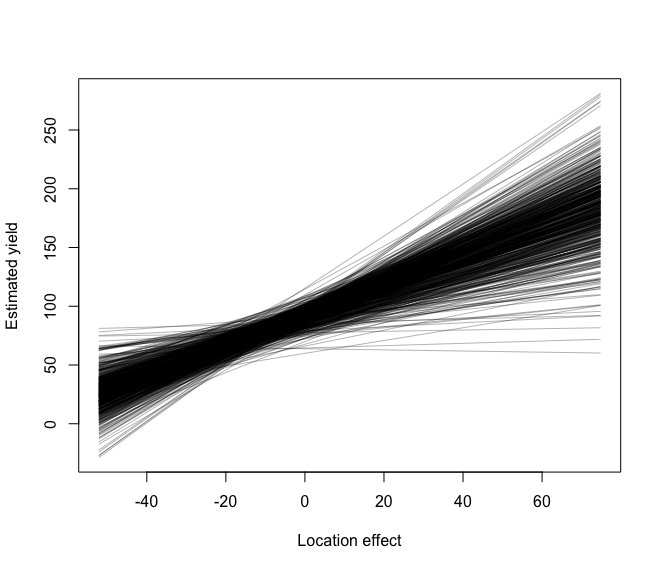
\includegraphics[width = 0.5\textwidth]{image8.png}
	\end{figure}
\end{frame}






\begin{frame}
	\frametitle{Residuals of FW Model for Two Fields}
	\textbf{Problem:} the residuals are \textbf{highly spatially correlated}.
	\begin{figure}[H]
		\centering
		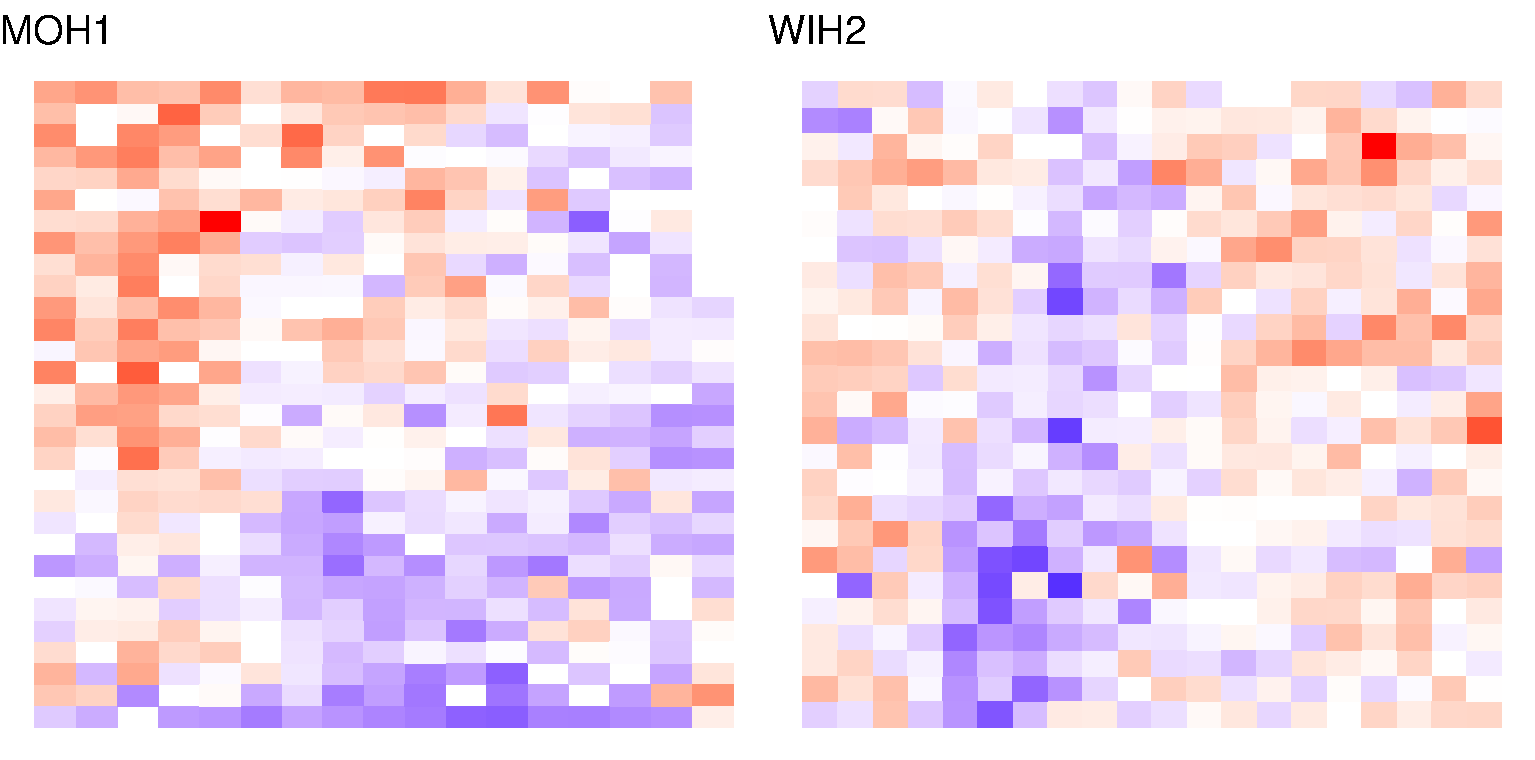
\includegraphics[width = 0.91\textwidth]{resid_plot_2.pdf}
	\end{figure}
\end{frame}



\begin{frame}
	\frametitle{Hierarchical Spatial Finlay-Wilkinson (SFW) Model}
	\begin{itemize}
	\item Data model:
\begin{equation*}
[y_{ijk} | \mu, \mathbf{g}, \mathbf{b}, \mathbf{h}, \bphi ] \ \ \overset{indep}{\sim} \ \  \mathcal{N}(\mu + g_i + h_j + b_i h_j + \phi_{ijk}, \sigma_e^2),
\end{equation*}

	\item Prior distributions for genotype, slope, and field effects:
	$$  [\mathbf{g}] \sim \mathcal{N}(\bm{0}, \bA \sigma_g^2); \ \ \ \ [\mathbf{b}] \sim \mathcal{N}(\bm{0}, \bA \sigma_b^2); $$
        $$[\mathbf{h}|\bm{\gamma}] \sim \mathrm{N}( \gamma_1 \bZ_1 + \dots + \gamma_l \bZ_l + \dots + \gamma_L \bZ_L
         , \mathbf{I} \sigma_h^2).$$
         \item $\bA$ is the kinship matrix describing the correlation structure of $\mathbf{g}$ and $\mathbf{b}$ \textcolor{blue}{(R package/software: rrBLUP, Tassel 5)}.
	\item $\bZ_{l}$ is the $l$th standardized environmental covariate.
	\end{itemize}
\end{frame}


\begin{frame}
	\frametitle{Intrinsic Autoregression Model for Spatial Effects}
	\begin{itemize}
	\item A popular model for fertility adjustment in agricultural field trials is the \textbf{first order intrinsic autoregression} \citep{besag1999bayesian,dutt:mond:2015}.

\item First order Intrinsic Autoregressive prior:

\begin{equation*}
[\bpsi_j|\theta_j,\sigma^2_j] \propto |\sigma^{-2}_j\bW_j|_+^{1/2}\exp\left( -\shalf\sigma^{-2}_j\bpsi_j\bW_j\bpsi_j\right)
\end{equation*}
where
\[\bpsi_j\bW_j\bpsi_j = \theta_j\sum\sum(\psi_{u,v} - \psi_{u-1,v})^2 + {\bar\theta}_j\sum\sum(\psi_{u,v} - \psi_{u,v-1})^2\]

\item  The distribution of $\pmb{\psi}_j$ is \textbf{invariant} to the addition of arbitrary constant.

	\end{itemize}

\end{frame}




\begin{frame}
	\frametitle{Intrinsic Autoregression Model for Spatial Effects}

\textcolor{blue}{Recall: } 
\begin{itemize}
\item $[y_{ijk} | \mu, \mathbf{g}, \mathbf{b}, \mathbf{h}, \bphi ] \ \ \overset{indep}{\sim} \ \  \mathcal{N}(\mu + g_i + h_j + b_i h_j + \phi_{ijk}, \sigma_e^2), $
\end{itemize}

\pause
	
\textcolor{blue}{Problem: }
\begin{itemize}
\item The intrinsic spatial prior has an \textbf{indeterminate overall level}.
\item The overall levels of \textbf{spatial effects} are \textbf{confounded with} the \textbf{location effects}.
\item Estimation of $\mathbf{b}$ is biased.
\item Hierarchical structure of $\mathbf{h}$ is not applicable.
\end{itemize}

\pause
\textcolor{blue}{Solution: }
	\begin{itemize}
\item  \textbf{A hard constraint}:  set the average of the spatial effects to zero.
\end{itemize}
 
\end{frame}




\begin{frame}
	\frametitle{Projected Intrinsic Autoregression (PIAR) Prior}

  	\begin{itemize}
	\item The Gaussian projected intrinsic autoregression (PIAR) on the $r_j \times c_j$ regular array is then defined as:
	\begin{equation*}
\bphi_j = \bB_j \bvarphi_j,\qquad \bvarphi_j\sim{\mathcal N}(\mathbf{0},\bD_j^{-1}),
\end{equation*}
\item  $\bB_{j}$ is an $r_jc_j \times (r_jc_j-1)$ matrix.
\item $\bD_j$ is an $(r_jc_j-1) \times (r_jc_j-1)$ diagonal matrix. 
\item We can show: $\bvarphi_j = \bB_j^\sT \bphi_j$.
	\end{itemize}
	
\end{frame}









\begin{frame}
	\frametitle{Matrix Free Computation}
	
	\begin{itemize}
	\item  The covariance matrix of the Gaussian PIAR is a \textbf{dense} singular matrix.
	\item The computation load for generating $\bphi_j$ from PIAR using knowledge of multivariate statistics is ${\mathcal O}((r_jc_j)^3/3)$.
	\item Assume \textbf{small number of missing plots} (denote $r_j c_j-N_j$ as the number of missing plots).
	\item Thus matrix-vector multiplications with $\bB_j$ and $\bB^{\sT}_j$ can also be performed using these \textbf{discrete cosine transformations (DCT)}.
	\item The computation load of our proposed algorithm is $\mathcal{O}( r_jc_j + (r_j c_j-N_j) r_j c_j \log r_jc_j +  (r_j c_j-N_j)^3/3)$.	\end{itemize}
	
\end{frame}





\begin{frame}
	\frametitle{Prediction}
	
	\begin{itemize}
	\item Implement \textbf{posterior predictive distributions}.
	\item Easy to obtain predictive credible intervals.
	\end{itemize}
	\pause
	\textcolor{blue}{Within-field prediction}:
	\begin{itemize}
	\item Important to account for the spatial correlation between plots.
	\item Kinship information plays a decisive role for an accurate prediction.
	\item Mainly used for \textbf{model evaluation}.
	\end{itemize}
	\pause
	\textcolor{blue}{Predict in new environments}:
	\begin{itemize}
	\item By learning how environment effects depend on the weather and soil variables.
	\end{itemize}
	
\end{frame}



\begin{frame}
	\frametitle{Model Evaluation via Within-Field Prediction}
	Reduced error for yield prediction.
	\begin{figure}[H]
		\centering
		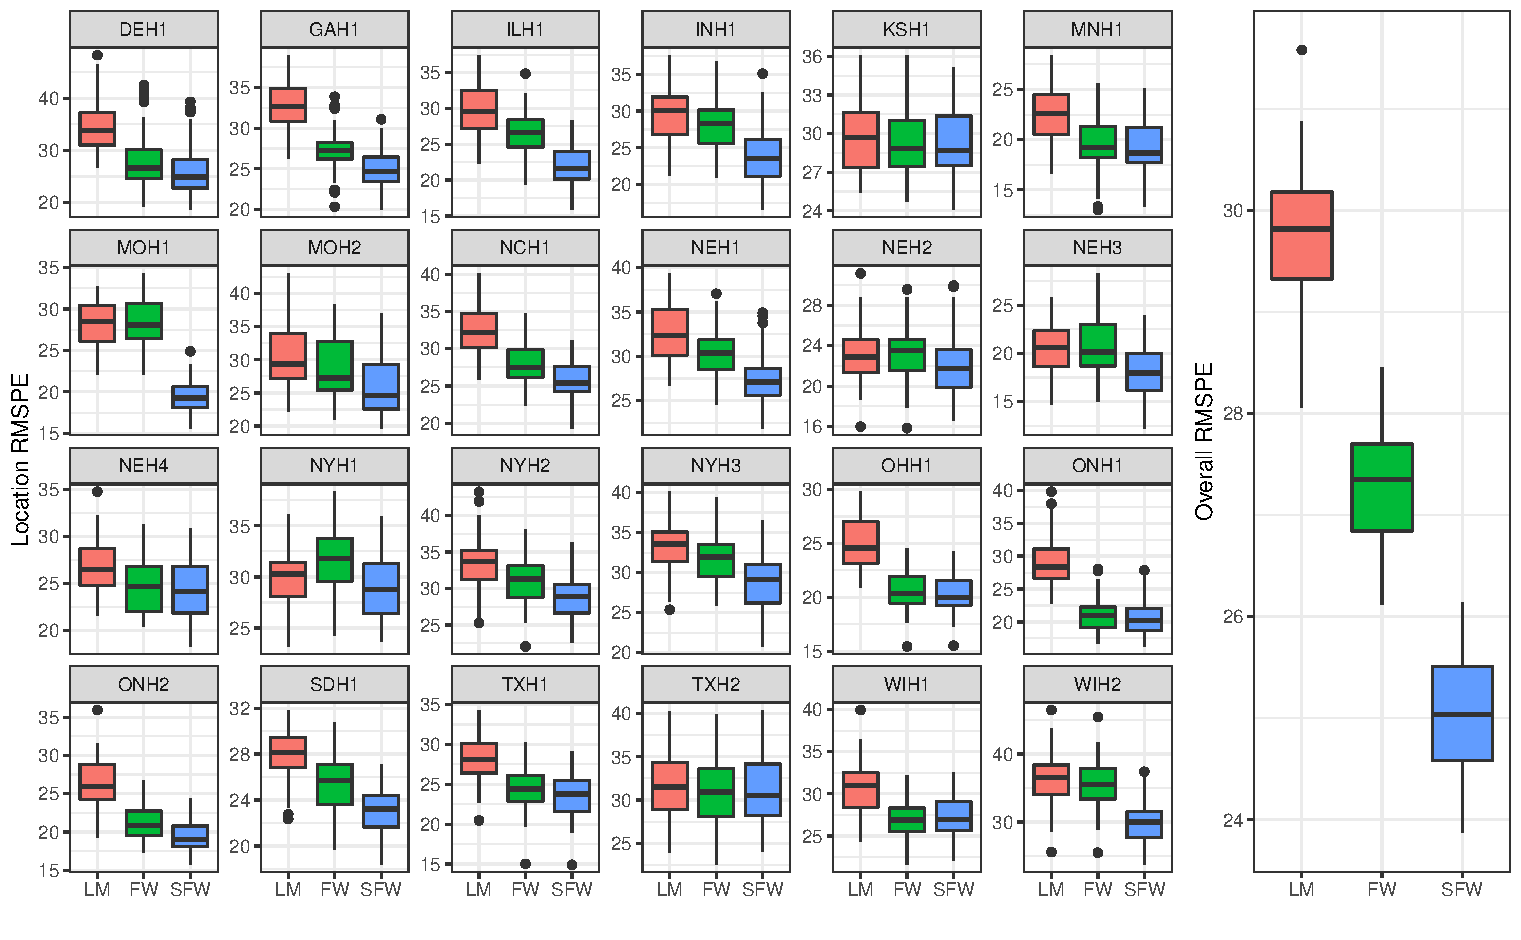
\includegraphics[width = 0.9\textwidth]{com_pred3.pdf}
	\end{figure}
\end{frame}



\begin{frame}
	\frametitle{Model Evaluation via Within-Field Prediction}
Level of spatial correlation vs performance of SFW model.

	\begin{figure}[H]
		\centering
		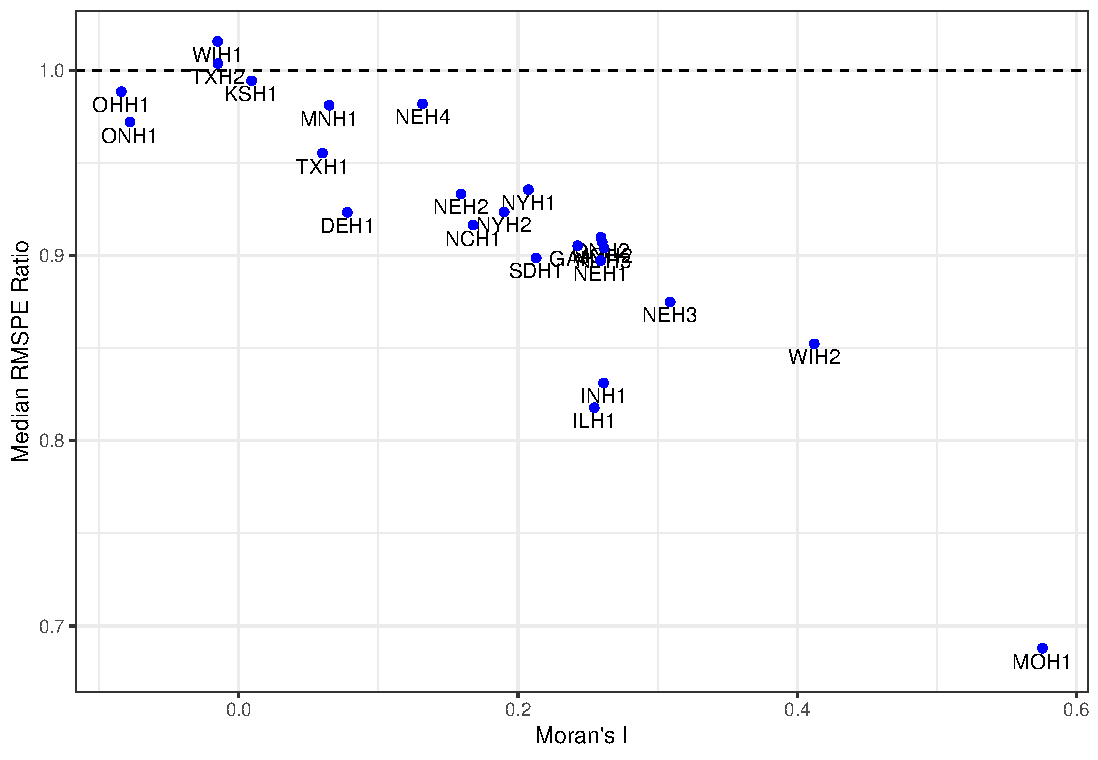
\includegraphics[width = 0.8\textwidth]{morans_i.pdf}
	\end{figure}
\end{frame}


\begin{frame}
	\frametitle{Prediction Intervals}
	50 plot yield prediction intervals ($95\%$ credible level).
	\begin{figure}[H]
		\centering
		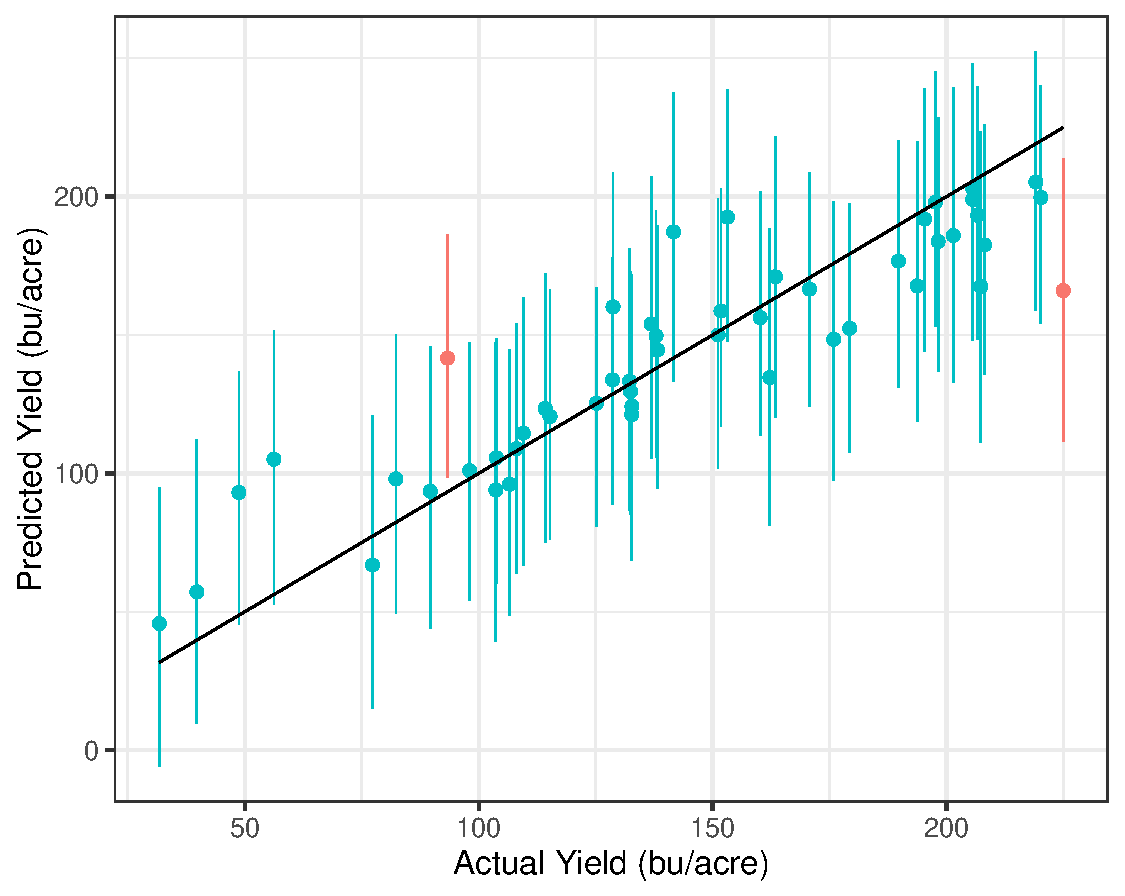
\includegraphics[width = 0.75\textwidth]{true_vs_predint.pdf}
	\end{figure}
\end{frame}




\begin{frame}
	\frametitle{Predict in New Environments}
	Location-wise RMSPEs computed using temperature and rainfall data (x-axis), versus the location-wise RMSPEs computed not using any environment information (y-axis). 
	\begin{figure}[H]
		\centering
		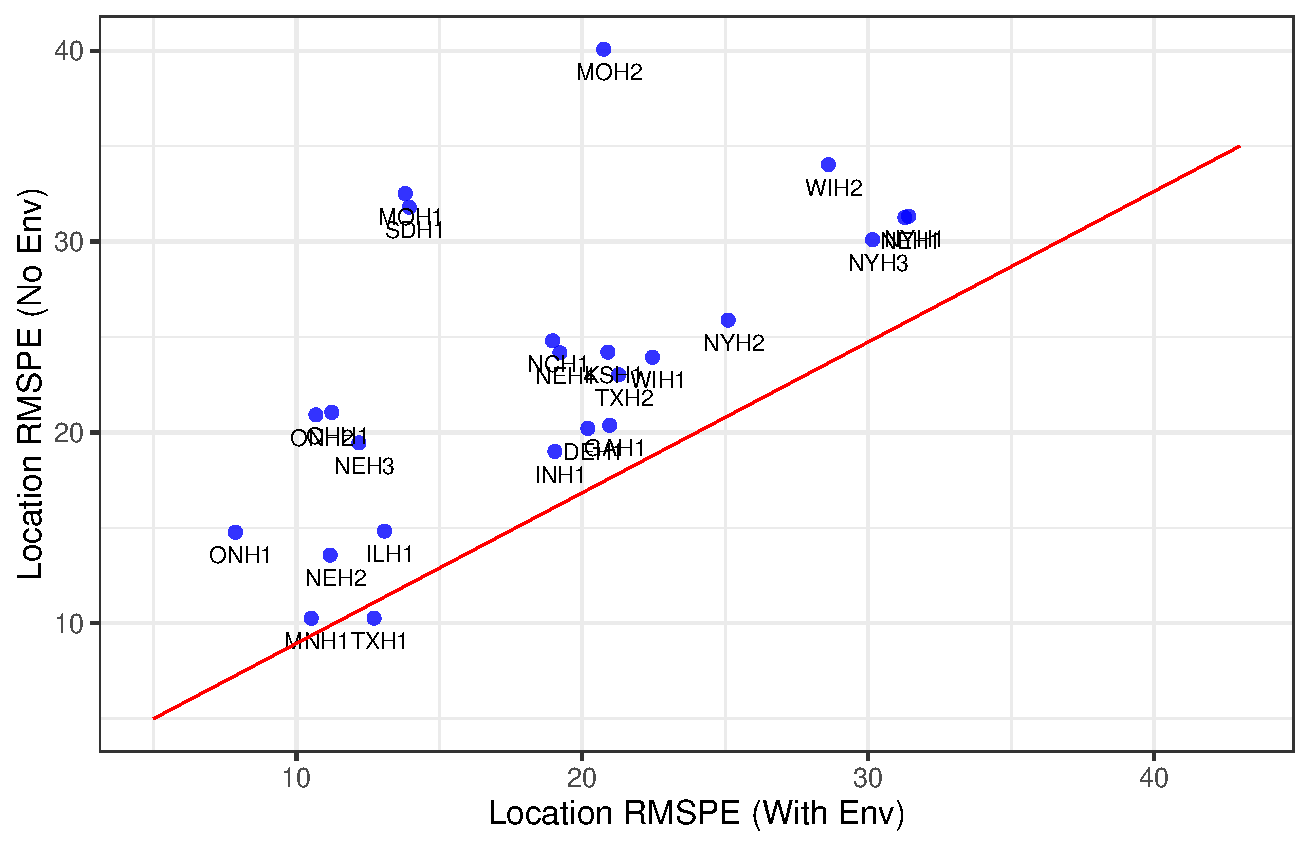
\includegraphics[width = 0.8\textwidth]{type3pred1.pdf}
	\end{figure}
	
\end{frame}







\begin{frame}
\frametitle{Selected References}
\bibliographystyle{apalike}
\bibliography{FWspatial}
\end{frame}



\begin{frame}
\frametitle{Acknowledgements}
The authors acknowledge financial support of Iowa State University Plant Sciences Institute Scholars Program, the Baker Center for Bioinformatics and Biological Statistics, and the Iowa Agriculture and Home Economics Experiment Station, Ames, Iowa, Project No. IOW03617, which is supported by USDA/NIFA and State of Iowa funds. 


Any opinions, findings, conclusions, or recommendations expressed in this publication are those of the authors and do not necessarily reflect the views of the U.S. Department of Agriculture.
\end{frame}




\begin{frame}%%     1
\begin{center}
\Huge Thank You!
\end{center}
\end{frame}




\begin{frame}
	\frametitle{Construction of $\bB_{j}$ and $\bD_j$}

  	\begin{itemize}
         \item Then the spectral decomposition of $\bW_j$ is given by:
         $$( \bN_{r_j}\otimes\bN_{c_j}) \bW_j ( \bN_{r_j}^\sT \otimes\bN_{c_j}^\sT) = \theta_j\bLambda_{r_j}\otimes\mathbf{I}_{c_j} + \bar\theta_j\mathbf{I}_{r_j}\otimes\bLambda_{c_j}.$$
         \item $\bLambda_k$ denote the $k\times k$ diagonal matrix  whose $u$th diagonal entry is $4\sin^2\{\pi(u-1)/(2k)\}.$
	\item $\bN_k$ denotes the $k\times k$ orthogonal matrix whose $(u,v)$th entry is $1/\sqrt{k}$ if $u=1,$ $\forall v,$ and $(2/k)^{1/2}\cos\{\pi(u-1)(v-1/2)/k\}$ otherwise.
	\item  $\bB_{j}^{\sT}$ denotes the $(r_jc_j-1)\times r_jc_j$ matrix consisting of last $r_jc_j-1$ rows of $ \bN_{r_j}\otimes\bN_{c_j}$.
         \item $\bD_j$ denotes the diagonal matrix consisting of the nonzero elements of $\theta_j\bLambda_{r_j}\otimes\mathbf{I}_{c_j} + \bar\theta_j\mathbf{I}_{r_j}\otimes\bLambda_{c_j}$.
	\end{itemize}
	
\end{frame}




\begin{frame}
	\frametitle{Assessing Uncertainty about FW Regression Lines}

\begin{figure}[H]
  \begin{subfigure}{0.3\textwidth}
    \centering
    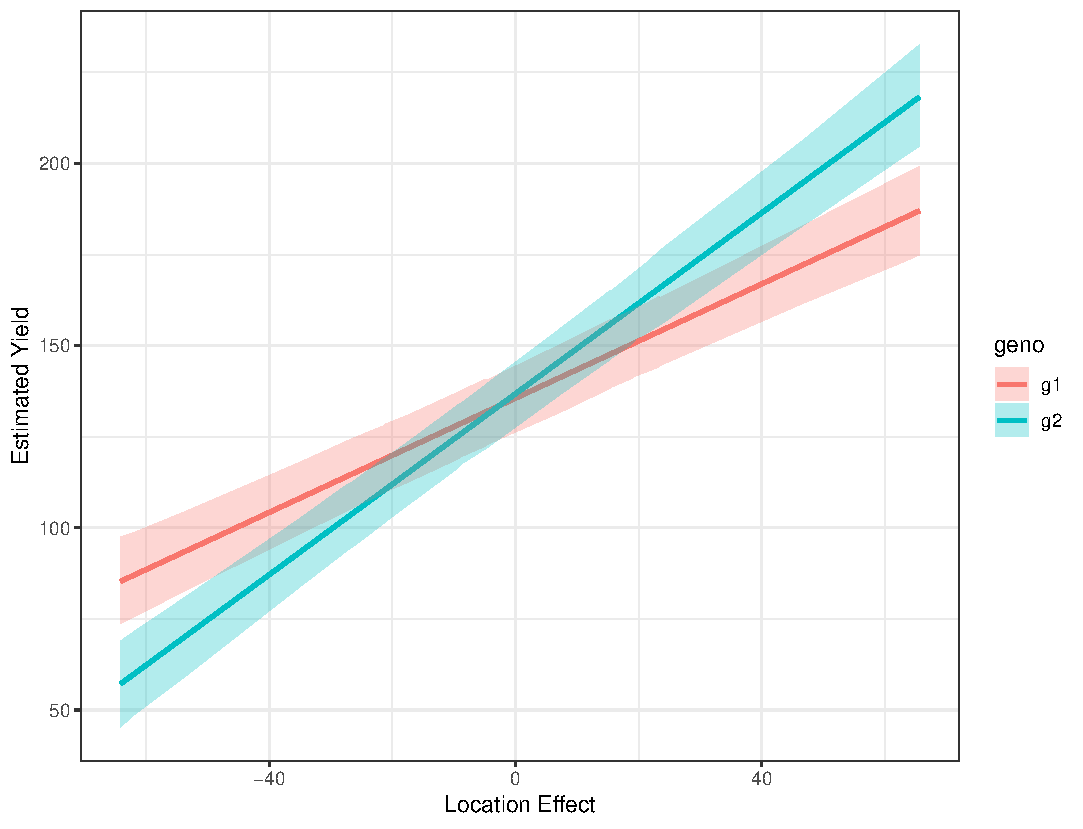
\includegraphics[width=.9\linewidth]{fwpair_1.pdf}
    \caption{}
  \end{subfigure}%
  \begin{subfigure}{0.3\textwidth}
    \centering
    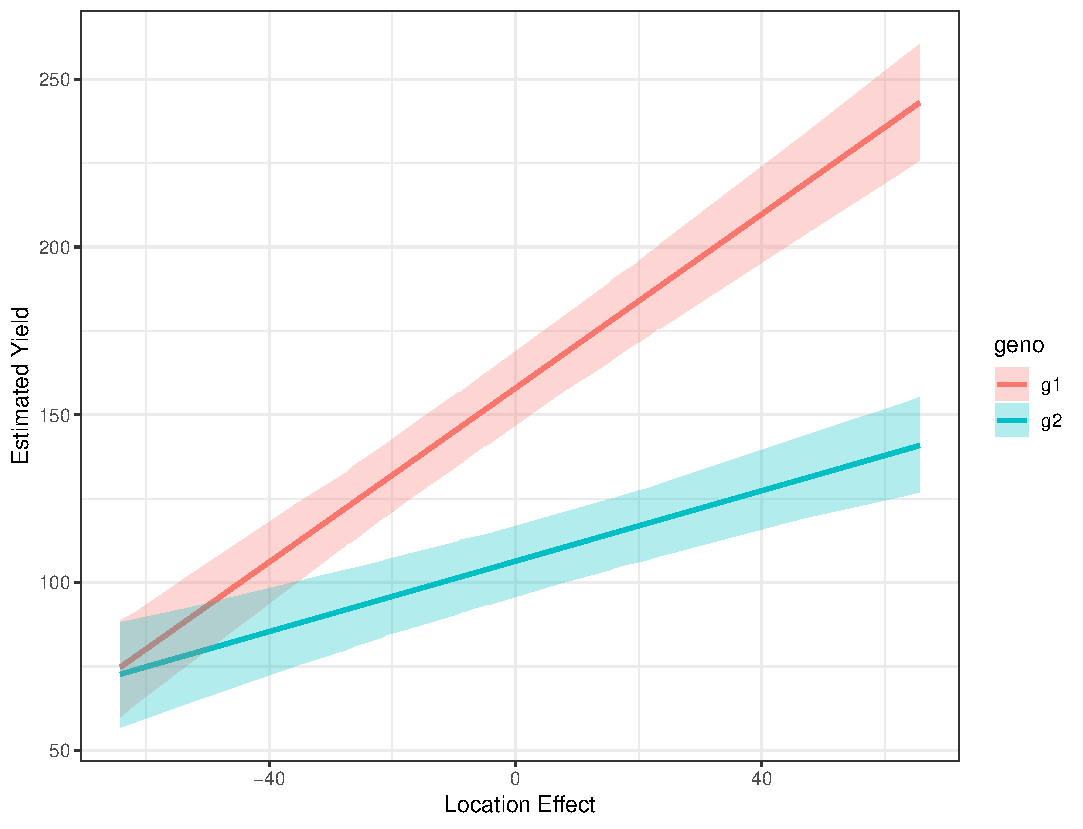
\includegraphics[width=.9\linewidth]{fwpair_2.pdf}
    \caption{}
  \end{subfigure}
  \begin{subfigure}{0.3\textwidth}\quad
    \centering
    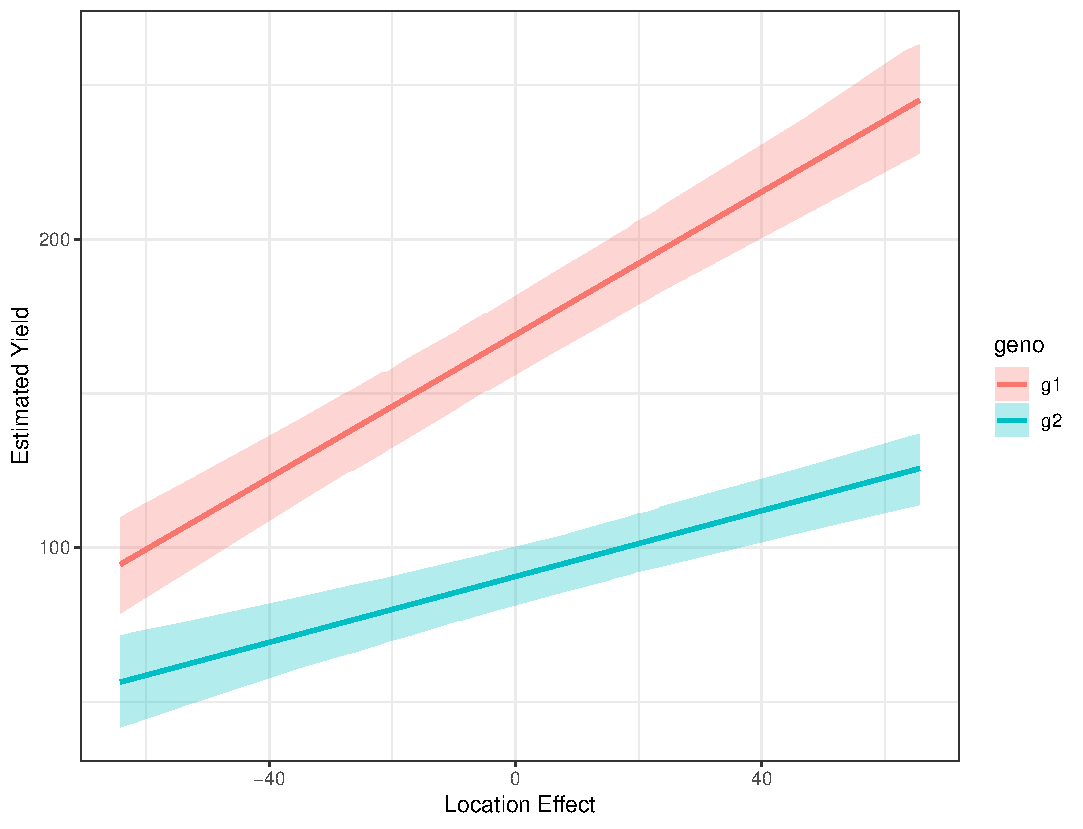
\includegraphics[width=.9\linewidth]{fwpair_3.pdf}
    \caption{}
  \end{subfigure}
  \medskip

  \begin{subfigure}{0.3\textwidth}
    \centering
    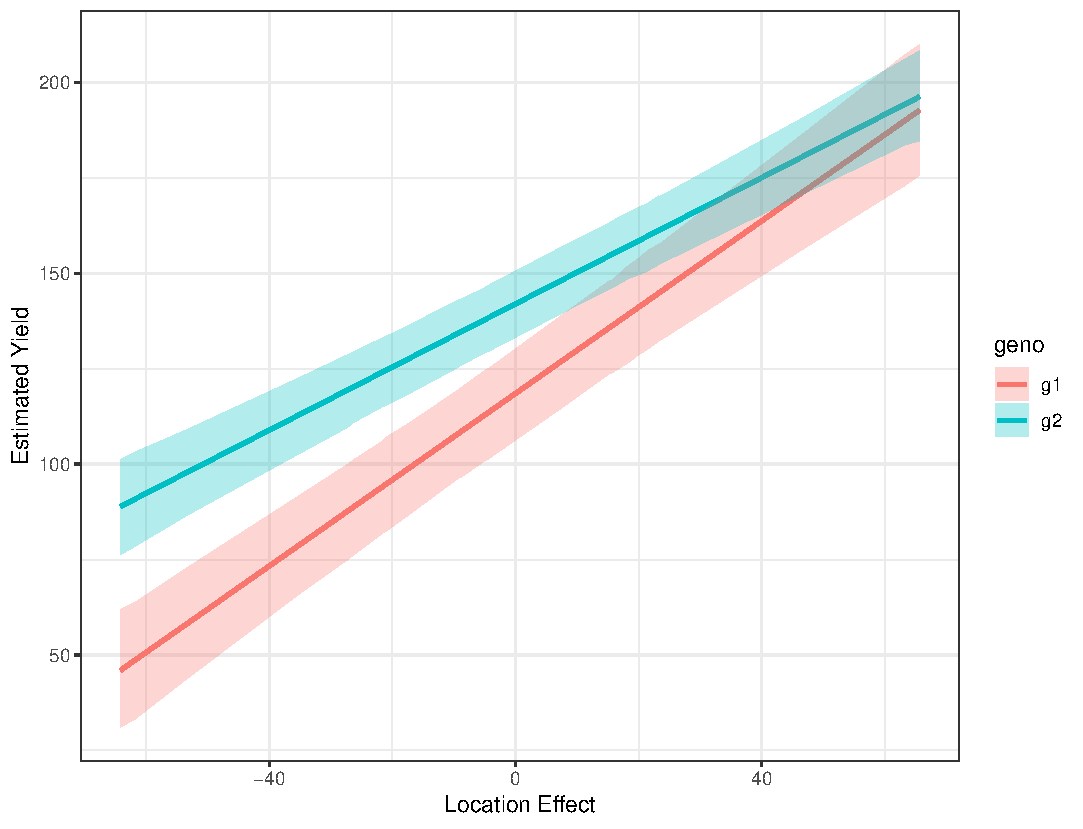
\includegraphics[width=.9\linewidth]{fwpair_4.pdf}
    \caption{}
  \end{subfigure}
  \begin{subfigure}{0.3\textwidth}
    \centering
    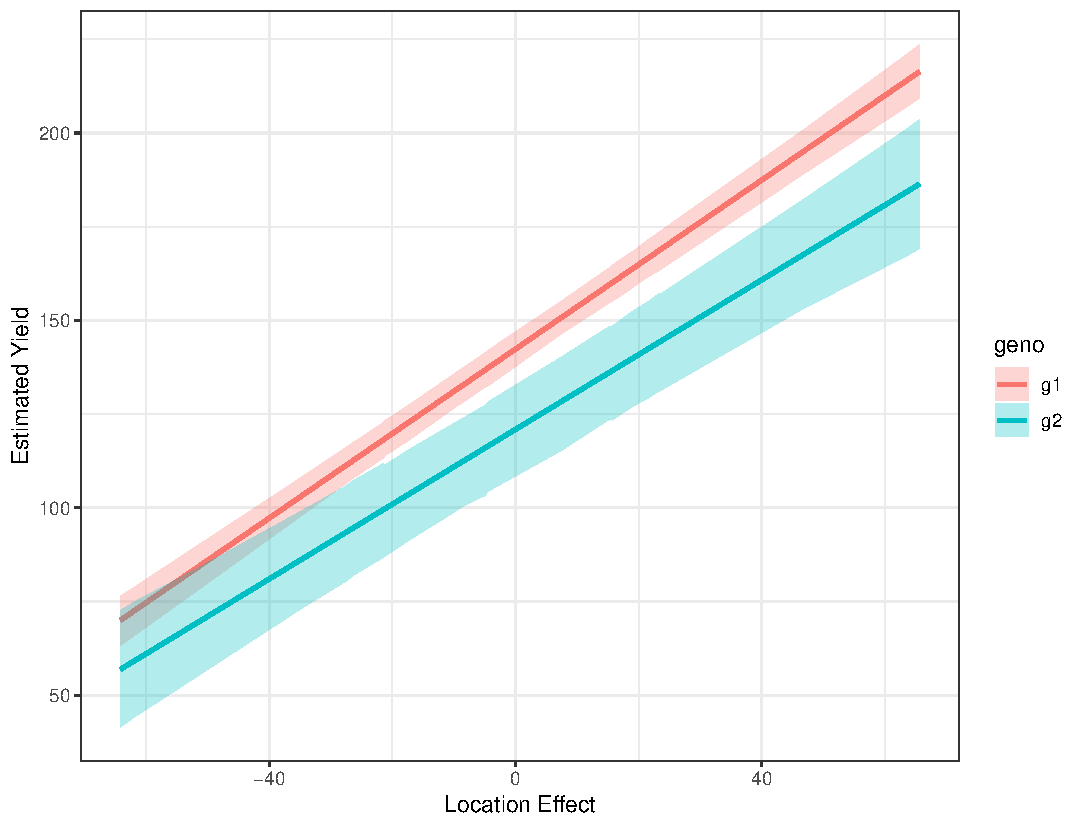
\includegraphics[width=.9\linewidth]{fwpair_5.pdf}
    \caption{}
  \end{subfigure}

  \caption{Estimated Yield vs Location Effect for pairs of genotypes}
\end{figure}


\end{frame}







\end{document}



